\documentclass[a4paper]{article}

%% Language and font encodings
\usepackage[english]{babel}
\usepackage[utf8x]{inputenc}
\usepackage[T1]{fontenc}

%% Sets page size and margins
\usepackage[a4paper,top=3cm,bottom=2cm,left=3cm,right=3cm,marginparwidth=1.75cm]{geometry}

%% Useful packages
\usepackage{amsmath}
\usepackage{graphicx}
\usepackage[colorinlistoftodos]{todonotes}
\usepackage[colorlinks=true, allcolors=blue]{hyperref}
\usepackage[listings]

\title{%
    Multi-Core Nested Depth-First Search\\
    \large ECE 5510 Course Project, Fall 2019}

\author{Annette Feng, Yuqing Liu}

\begin{document}
\maketitle


\begin{abstract}

Model Checking is a method for analyzing the finite-state model of a system for correctness against a given specification. A certain class of algorithms for exploring the state space in Model Checking employ Nested Depth-First Search. Depth-First Search algorithms are inherently sequential. The first \emph{multi-core} version of Nested Depth-First Search was introduced in~\cite{laarman} and has since been followed up by various improvements. In this paper, we present our exploration of Multi-Core Nested Depth-First Search (MC\_NDFS) algorithms for our ECE 5510 Course Project. We compare five different implementations of MC\_NDFS, including our own variation based on our observations of the other four.

\end{abstract}


\section{Introduction}

In Model Checking (MC), verification of the Linear Temporal Logic (LTL) property of liveness of a system specification is a non-trivial task, unlike that of safety which can be handled as a matter of reachability. The LTL MC problem is reducible to finding accepting cycles in a graph. This is accomplished through techniques employing Depth-First Search (DFS). The Nested Depth-First Search (NDFS) algorithm, as introduced in~\cite{ndfs}, solves this problem in linear time using a 2-phase recursive search process, with each phase visiting any state at most once. In the first phase, \emph{dfs\_blue}, the search process colors blue all states encountered as it looks for all the accepting states in its path. The second phase, \emph{dfs\_red}, is initiated from \emph{dfs\_blue} on all accepting states found, but in reverse order. The \emph{dfs\_red} search colors each state encountered red as it looks for any cycles around the accepting states. If the node \emph{s} that initiated the \emph{dfs\_red} search is encountered during this phase, \emph{s} is reachable from itself and \emph{dfs\_red} reports that a cycle has been detected. Because DFS is an inherently sequential operation, solutions involving these techniques must be carefully adapted to run correctly in Multi-Core (MC) environments.

This paper is organized as follows. In Section~\ref{background} we discuss the different MC variations of NDFS that we tested. In Section~\ref{implementation} we discuss the details of our implementation and testing procedure. In Section~\ref{experiments} we present our experiments and results. Finally, in Section~\ref{conclusion} we present our conclusions.


\section{Background}\label{background}

Swarm Verification (SV), mainly used in distributed memory environments, can be used to run NDFS algorithms in multi-core environments by adapting NDFS to use shared-state storage. This naive MC implementation has each thread traversing the complete state space, which can be stored in shared memory. Each thread independently performs a DFS, but using a unique order of successor states. This ensures that each thread explores a different part of the reachable state space first. However, this adaptation also results in the graph being explored \emph{N} times.

Variations of NDFS, based on observations of the feasible color combinations with which the states can be colored by the path-coloring scheme, allows for the early detection of cycles and pruning of the search space. A first variation of MC\_NDFS utilizes global coloring to share state among the threads~\cite{nndfs}. The basic idea is that when \emph{dfs\_red} backtracks, the states are globally marked red so that these states can be ignored by both red and blue searches, thus pruning the search space of other threads.

A second variation makes further improvements as suggested in~\cite{allred}. Here, the \emph{dfs\_blue} search adds an additional check: if all successors of a state \emph{s} are red, then \emph{s} can be colored red as well to avoid some calls to \emph{dfs\_red}.

In the next section we discuss our implementation of these three MC\_NDFS algorithms, in addition to two others, one that makes an improvement in the second variation, and the last variation being our own adaptation.


\section{Implementation}\label{implementation}

To run from the project directory, execute: \texttt{./bin/runtest} with no arguments to print usage information. The expected arguments are:

\begin{verbatim}
    <graph_size>
    <thread_count>
    <iterations>
    <num_graphs>
\end{verbatim}

We implemented the algorithms outlined in the preceding section using Java 8. The following subsections describe the details of each implemented algorithm.


\subsection{Graph Generation}

Because we didn't have access to the graph generation tools described in~\cite{laarman}, we implemented our own graph generator, loosely described as follows:

\begin{enumerate}
    \item Generate the initial graph as a tree structure with the root as the initial
        state. We recursively generate a variation of trees with a different ratio of
        nodes at each level by using a random number to decide the level-to-level ratio of nodes.  
    \item Add internal connections to produce cycles in the tree. To do that in a straightforward way,
        we randomly select two node and connect them. 
        The tree has $n-1$ edges for $n$ nodes, so, we randomly select a percentage $p$,
        and add $p\times n$ edges to the graph. The result indicates that a random $p$ between
        certain range can introduce from 0 to several cycles.
    \item Randomly mark a percentage of nodes as accepting.
        Although we can let the algorithm detect any cycle, we want to bring the benchmark close to what the algorithm expects. We select a small percentage of nodes to better randomize the chances of
        encountering cycles.
    
\end{enumerate}
    We used $40\%$ to $167\%$ downward level-to-level ratio for graph generation,
     $p = 10\%$ to $60\%$ to generate additional edges,
    and have $0.5\%$ to $3.5\%$ accepting nodes.
    As a result, we can generate about $50\%$ graphs with cycles.


\subsection{Naive\_MC\_NDFS}

The naive implementation is found in file \texttt{src/main/java/ndfs/RB2\_Thread.java}. Each thread is initialized with a \texttt{ThreadLocal} \textt{HashMap} to store the visited states along with their set color. For this, as well as all other variations that we describe, the initial coloring of each state is \texttt{WHITE}. Because the threads in the naive implementation operate independently, we expect this version to show the worst performance, as the entire state space is explored $\text{N}$ times, where $\text{N = \emph{thread\_count}}$.


\subsection{MC\_GC\_NDFS: Global Color Variation}

The first variation is found in file \texttt{src/main/java/ndfs/MC\_NDFS\_Thread.java}. In this version, a thread globally colors states red when \texttt{dfs\_red} backtracks. This signals both red and blue searches that these states can be ignored, allowing other threads to prune them from their searches. We attach this variable, as well as a global \texttt{count} variable to each state, or node. The \texttt{count} variable is used to count the number of threads that have initiated a \texttt{dfs\_red} search on state \emph{s}.


\subsection{MC\_AR\_NDFS: AllRed Variation}

The second variation is found in file \texttt{src/main/java/ndfs/MC\_NDFS2\_Thread.java}. This version keeps the improvements of the first variation but adds a check in the blue search to ignore successor states that are colored red in order to prune the search.


\subsection{MC\_RS\_NDFS: RedSet Variation}

The third variation is found in file \texttt{src/main/java/ndfs/MC\_CNDFS\_Thread.java}. In this version, when a red search is initiated on seed node \emph{s}, the node collects all reachable states and, if no cycle is found, waits for any and all non-red nodes in the set to become red, as they eventually will because no cycles had been detected during the red search.


\subsection{MC\_NEW\_NDFS: Our Variation}

The final variation is our own variation which can be found in file:

\begin{verbatim}
    src/main/java/ndfs/NEW_Thread.java
\end{verbatim}

We saw that the AllRed variation has the best performance when there is no cycle,
so we want to try to improve it in some other way.

Our observation is that AllRed can detect if the connecting nodes of a node are red or not faster than the RedSet variation. Marking a node red means that there is no cycle
that contains the node and an accepting node. In the AllRed variation, non-accepting nodes are marked red before \texttt{dfs\_red} returns, and in the RedSet variation only marks a node red after an entire red search from the \texttt{dfs\_blue} is finished. As the path branches in each node, RedSet marks a node red relatively late, and we observed 2x speedup for AllRed comparing to any other variation.

In RedSet, an optimization is that when a \texttt{dfs\_blue} call finishes its calls on its successors, it prevents other threads from calling \texttt{dfs\_blue} on the node. We believe this is helpful, since at this stage the only thing left for the \texttt{dfs\_blue} call to do is initiate the red search. This seems expensive for the RedSet variation since it involves the usage of a set. 

We can use a similar mechanism to improve the performance of other variations, so we chose the AllRed implementation and attached the mechanism on it. 
The correctness still holds since we still have at least one thread calling \texttt{dfs\_blue}
on the connections, and then the \texttt{dfs\_red} on the node itself.


\section{Results}\label{experiments}
We ran 900+ graphs on the algorithms such that each graph runs on
each algorithm for 5 iterations, and we take the average time consumption.
Graph generation is configured as stated in the graph generation section.

In Figure~\ref{fig:cycle1}, we can see some lines forming up as time consumption increases. We conclude that it is due to property of random generated graph.
The average speedup is 1.379, which meets our expectation that we can encounter some cycle sooner with more threads.

\begin{figure}[ht]
\centering
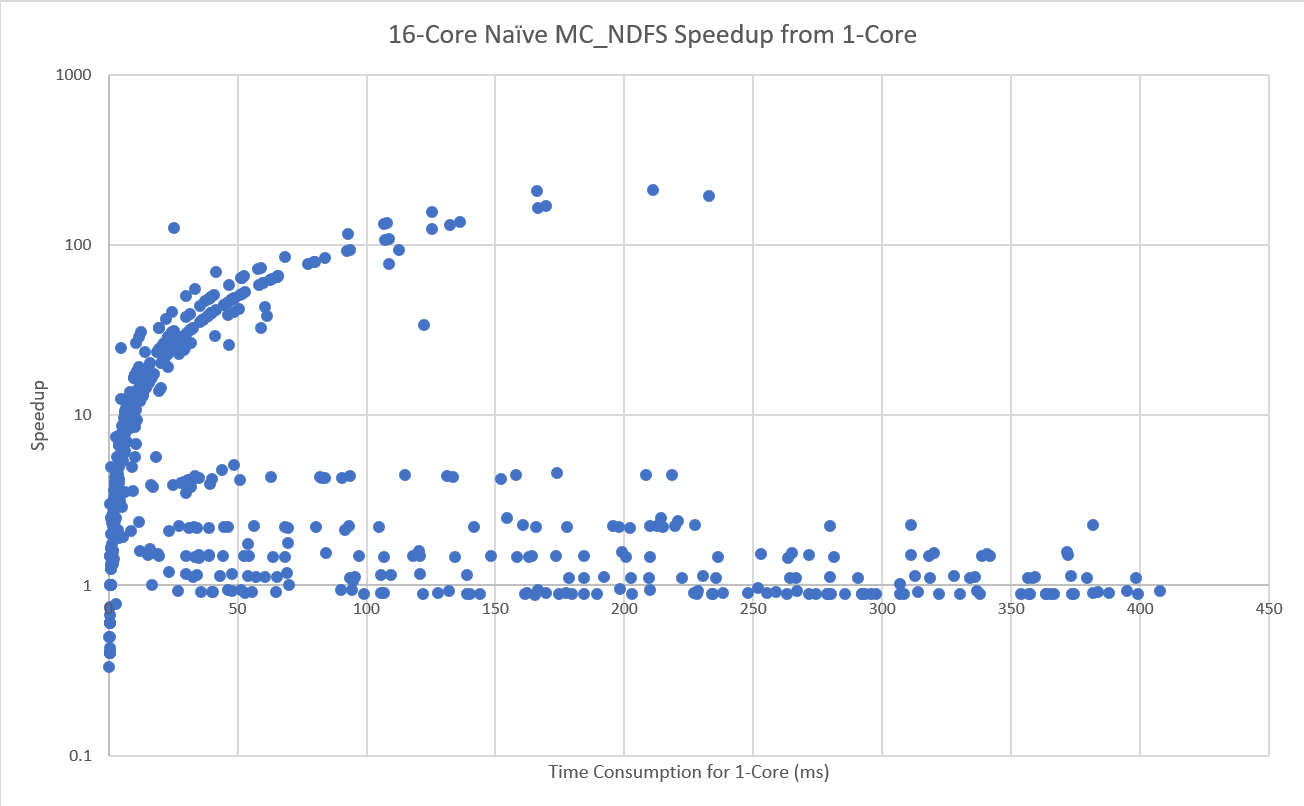
\includegraphics[width=0.75\textwidth]{cycle1.PNG}
\caption{\label{fig:cycle1}16-core Naive\_MC\_NDFS vs sequential with cycles.}
\end{figure}

\begin{figure}
\centering
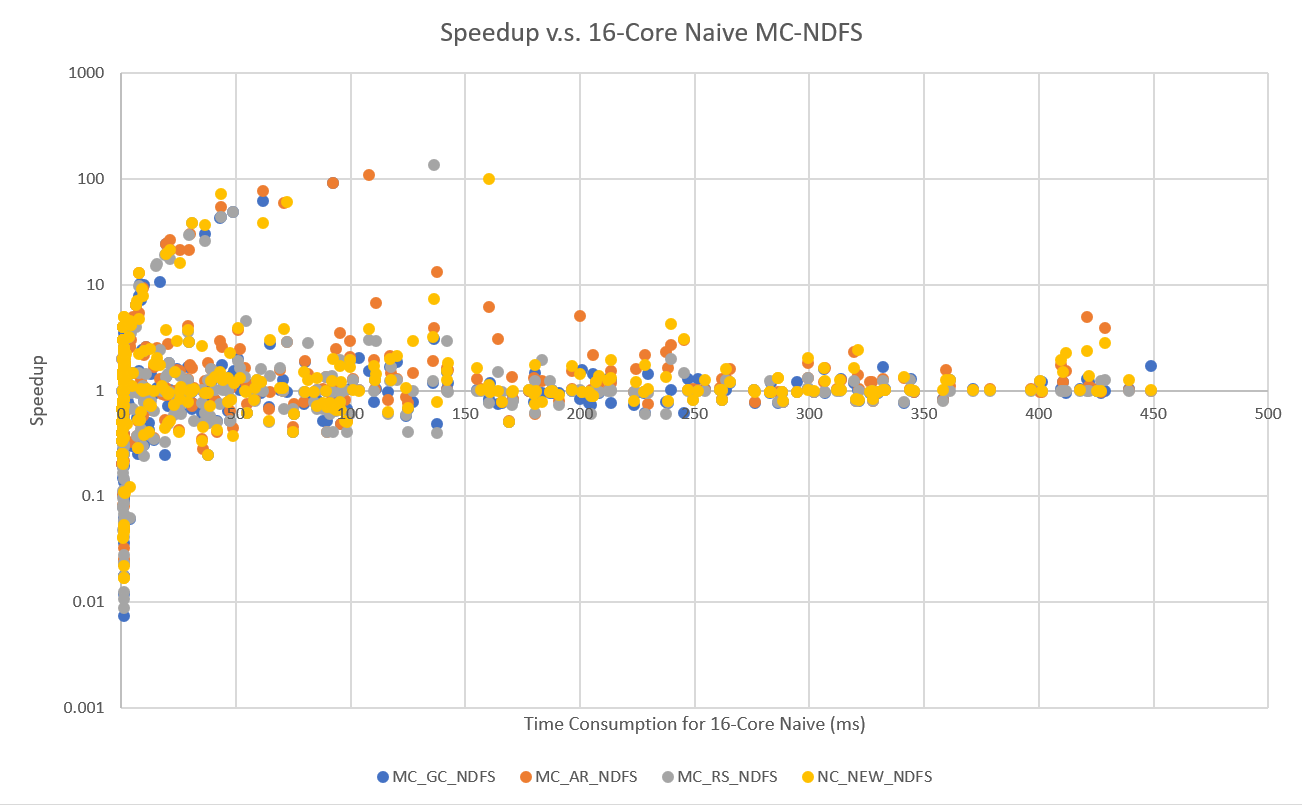
\includegraphics[width=0.75\textwidth]{cycle16.PNG}
\caption{\label{fig:cycle16}16-core tests over graphs with cycles.}
\end{figure}

\begin{figure}
\centering
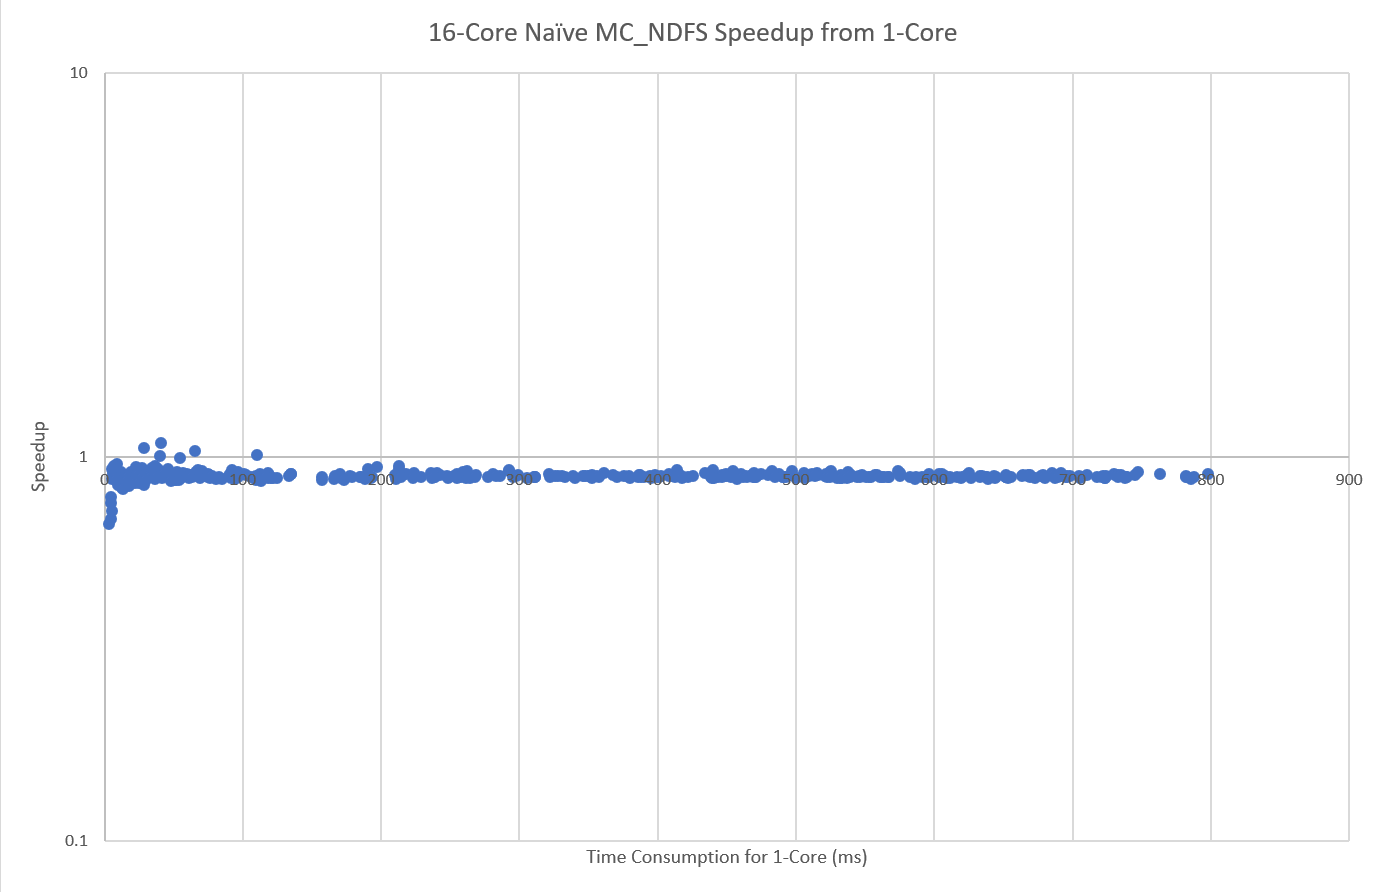
\includegraphics[width=0.75\textwidth]{nocycle1.PNG}
\caption{\label{fig:nocycle1}16-core Naive\_MC\_NDFS vs sequential without cycles.}
\end{figure}

\begin{figure}
\centering
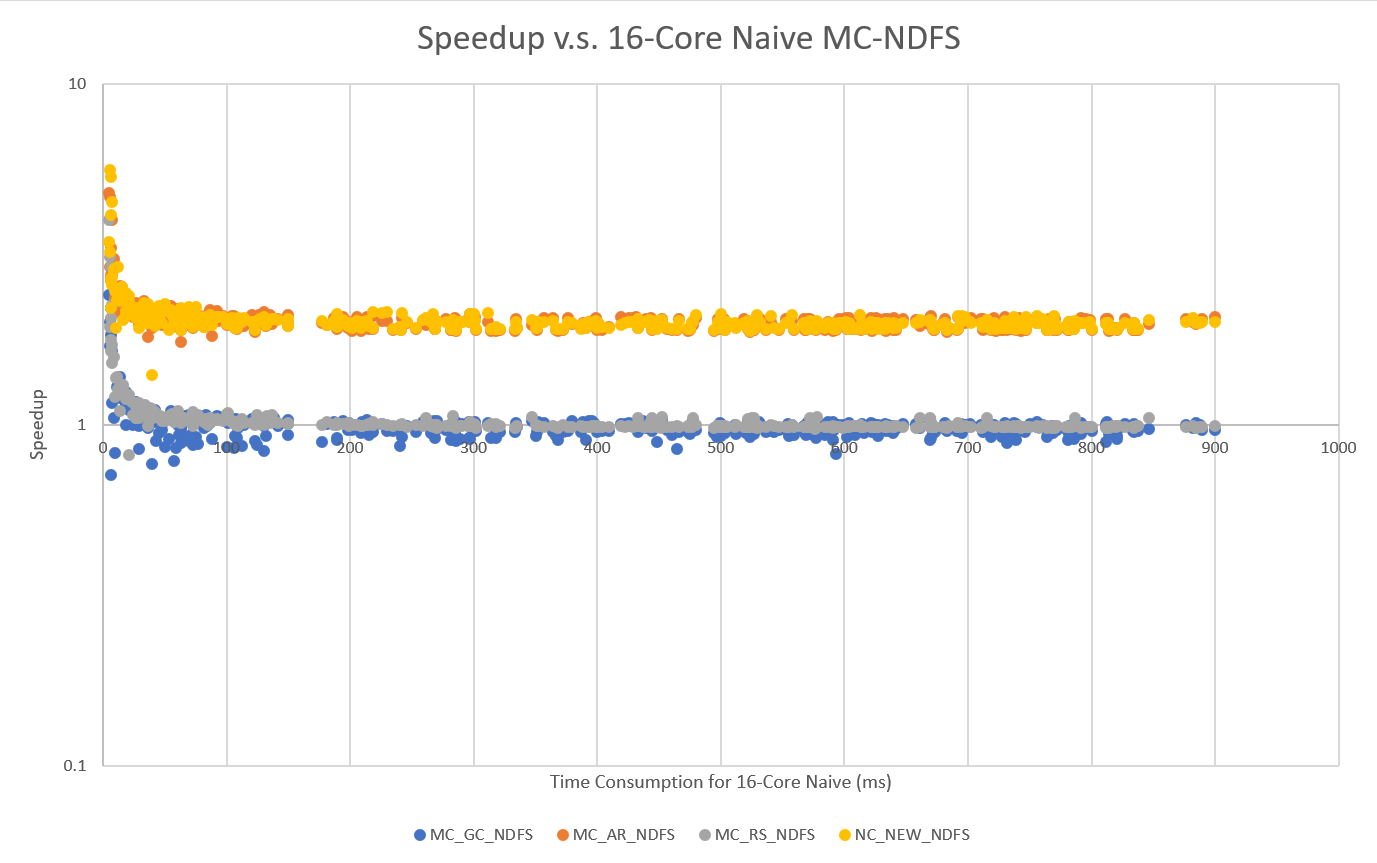
\includegraphics[width=0.75\textwidth]{nocycle16.PNG}
\caption{\label{fig:nocycle16}16-core tests over graphs without cycles.}
\end{figure}

In Figure~\ref{fig:cycle16}, we can see the improvement is relatively small from the 16-core naive implementation, which is a speedup of 1.3794. Since threads can encounter a cycle at a random time, we can see that there are chances for the improved variants to perform worse than the 16-Core Naive implementation.

The average speed up for MC\_GC\_NDFS is 0.9572, for MC\_AR\_NDFS is 1.1175, for MC\_RC\_NDFS is 0.9377, and for MC\_NEW\_NDFS is 1.0887. Two of the variants perform worse than the 16-Core baseline, which we believe is due to more collision between threads and the overhead introduced by accessing concurrent objects. The MC\_AR\_NDFS performs little better, which we think is due to preventing a thread from running \texttt{dfs\_red}. Our new implementation is also slightly better than the naive 16-Core baseline, but not as good as MC\_AR\_NDFS. 
We think this is because the optimization idea we obtained from MC\_RC\_NDFS is not
actually improving the performance, which is indicated by MC\_RC\_NDFS result.

Similarly in single core setting, the overhead of accessing multiple parts of the graph damages the 16-Core naive implementation's performance, resulting in a speedup of 0.8903, showing in Figure~\ref{fig:nocycle1}. However, the MC\_AR\_NDFS overcomes this by the same mark-red algorithm, which shows speedup of 2. The average speed up for MC\_GC\_NDFS is 0.9717, for MC\_AR\_NDFS is 1.9723, for MC\_RC\_NDFS is 0.9944, and for MC\_NEW\_NDFS is 1.9733, which is shown in Figure~\ref{fig:nocycle16}. Our implementation has received the same benefit since it is based on the MC\_RC\_NDFS, but it does not improve from there since MC\_RC\_NDFS doesn't shown improvement in speed.



\section{Conclusion}\label{conclusion}

We have presented several implementations of MC\_NDFS that show improvement over the sequential implementation of NDFS. We tried to improve the performance of the best-performer, MC\_RC\_NDFS, with some insight gained from our observations of our test results and from our understanding of the various algorithms. However, in the end, our implementation yielded no observable improvement over the MC\_RC\_NDFS algorithm. We have also seen the linear-like results in the cycle speedup plot, which indicates cycles can sometimes be found very quickly. We think this has something to do with the characteristics of the graph, and the randomization may happen to run into some cycles right away for all of our 5 iterations per graph per algorithm.

Our code is available on GitHub at:

\begin{verbatim}
    https://github.com/NAP64/Multicore_Nested_Depti-First_Search.git
\end{verbatim}


%%\LaTeX{} is great at typesetting mathematics. Let $X_1, X_2, \ldots, X_n$ be a sequence of independent and identically distributed random variables with $\text{E}[X_i] = \mu$ and $\text{Var}[X_i] = \sigma^2 < \infty$, and let
%%\[S_n = \frac{X_1 + X_2 + \cdots + X_n}{n}
%%      = \frac{1}{n}\sum_{i}^{n} X_i\]
%%denote their mean. Then as $n$ approaches infinity, the random variables $\sqrt{n}(S_n - \mu)$ converge in distribution to a normal $\mathcal{N}(0, \sigma^2)$.

\bibliographystyle{alpha}
\bibliography{bibliography}

\end{document}